% ! TeX root = ...

\begin{frame}{Research Questions}
  \begin{backgroundblock} 
    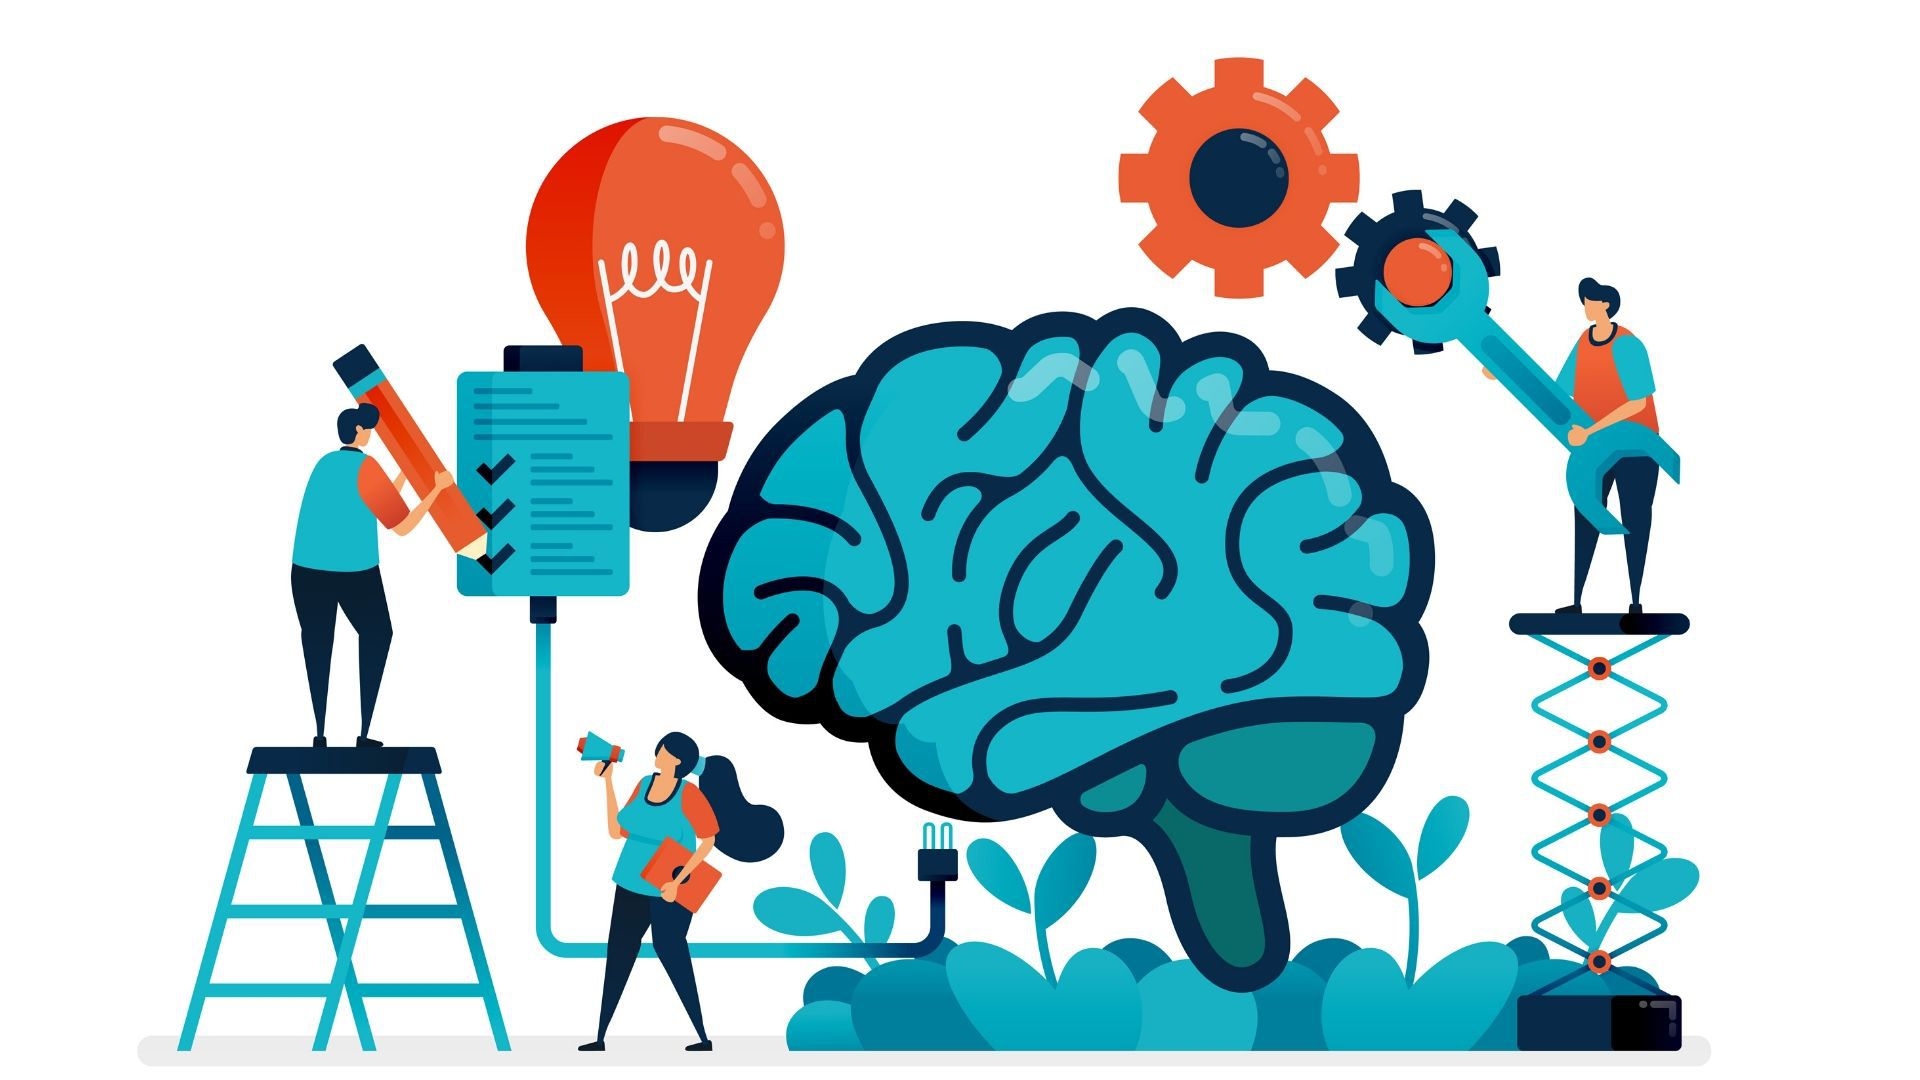
\includegraphics[width=\paperwidth]{img/background.jpg} 
  \end{backgroundblock} 
  \begin{card}
    \begin{itemize}
      \item[\faQuestion] <1-> What kind of Machine Learning approach is useful in combination with Aggregate Computing
      \item[\faQuestion] <2-> At what level of abstraction can Machine Learning be useful for Aggregate Computing
      \item[\faQuestion] <3-> What does Aggregate Computing have in common with Machine Learning, applied to Collective Self-Adaptive System
    \end{itemize}  
  \end{card}
  \pdfcomment 
  {
    The research question we want to tackle are: 
    i) what kind of machine learning is useful in combination with Aggregate Computing? 
    ii) at what level of abstraction can Machine Learning be useful for Aggregate Computing? 
    iii) what does Aggregate Computing have in common with ML, applied to Collective Adaptive System? 
    To do this we experiment with different cases of study that I'm going to present to you  
  }
\end{frame}